\label{fundamentacaoteorica}

\section{Web Semantica}
A web foi criada para possibilitar o acesso, intercâmbio e recuperação de informações de maneira rápida e simples, seu crescimento exponencial e caótico fez com que a mesma se tornasse hoje um gigantesco repositório de documentos, o que dificulta a recuperação de informações. Até o momento, não existe nenhuma estratégia abrangente e satisfatória para a indexação de documentos por meio de “motores de busca” que seja coerente com uma estrutura linguística. \cite{SouzaAlvarenga2004a} Com o intuito de preencher esse gargalo semântico na busca por informações, surge a web semântica. Ela tem como objetivo incorporar significado às informações presentes na web, criando um ambiente onde agentes de software e usuários possam trabalhar de forma cooperativa e entender o significado (sentido) presente nos dados. \cite{BrandaoLucena2002} Um exemplo da deficiência da web atual pode ser identificada na busca realizada pelos sistemas de recuperação de informação, que usam palavras-chave nas buscas,onde apenas a similaridade e o número de ocorrências de certas palavras no conteúdo de documentos são levados em consideração e não a semântica presente naquela informação. \cite{SouzaAlvarenga2004a}. 

Segundo a definição feita do W3C\footnote{http://www.w3.org/2001/sw}, a web semântica é um framework que permite compartir e reutilizar dados através das fronteiras das aplicações, empresas e comunidades. Ela tem duas funcionalidades principais: 

a) ser um conjunto de formatos para a integração e combinação de dados extraídos de diversas fontes, e; 

b) estabelecer uma linguagem para registrar como esses dados se referem a objetos do mundo real. 


\begin{figure}[!htb]
    \centering
    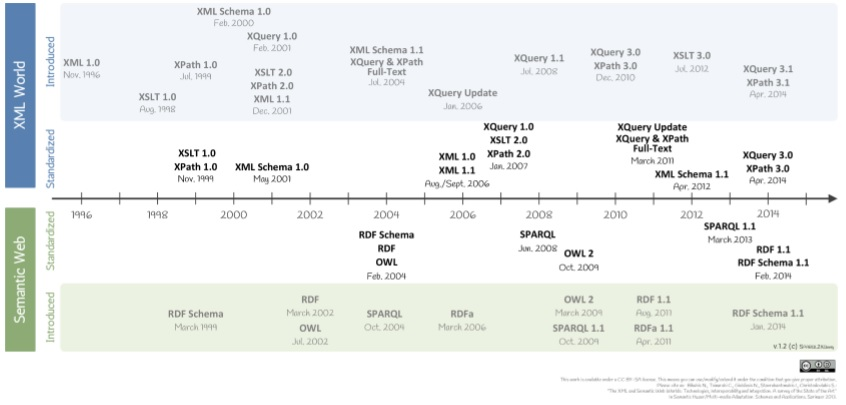
\includegraphics[width=12cm]{HistoriaWebSemantica.jpg}
    \caption{História da Web Semântica}
    \label{fig:HistoriaWebSemantica}
\end{figure}


A web semântica é formada por um conjunto de padrões propostos pelo World Wide Web Consortium (W3C). Eles evoluíram de padrões focados na representação de dados para a de conhecimento. Na \autoref{fig:HistoriaWebSemantica} podem ser observados os padrões que constituem a Web Semântica e sua relação com os padrões XML. Eles promovem formatos de dados comuns na WWW e também a inclusão de conteúdo Semântico na web, usando o padrão Resource Description Framework (RDF).

\section{Resource Description Framework}

O Resource Description Framework (RDF) é uma família de especificações da W3C, que foi disponibilizada em 1999 como parte do W3C Semantic Web Effort (Gruber, 1995). Ele foi originalmente projetado como um modelo de meta-dados e também chegou a ser usado como um método de descrições conceituais, principalmente para descrever recursos web. O RDF é usado em várias áreas de aplicação, como resource discovery para melhorar as capacidades dos motores de busca, cataloging para descrever o conteúdo e as relações de conteúdo disponibilizados em um sistema web particular, e descrição de intellectual property rights de páginas web. O modelo básico de dados consiste em um padrão de três tipos de objetos: 

\textbf{Sujeito:} representa os recursos e são identificados por meio de URIs, sem importar o tamanho deles, por exemplo, uma pagina web ou um elemento HTML podem ser recursos.

\textbf{Predicado:} são aspectos, características, atributos ou relações especificas que describem o sujeito, cada predicado têm um significado especifico e relaciona um sujeito com um objeto.

\textbf{Objeto:} um recurso especifico ou valor da propriedade que representa uma características do objeto\footnote{http://www.w3.org/TR/PR-rdf-syntax/}. 

Com RDF é possível explicitar relações entre dois objetos (usando-se uma Tripla RDF), mas não muito mais que isso. Para se descrever o que um objeto representa e suas relações com outros objetos, são necessárias ontologias.

\section{Ontologias}

A \autoref{fig:RepresentacaoOntologia} mostra os níveis de representação de dados na forma de conhecimento processável por máquinas.

\begin{figure}[!htb]
    \centering
    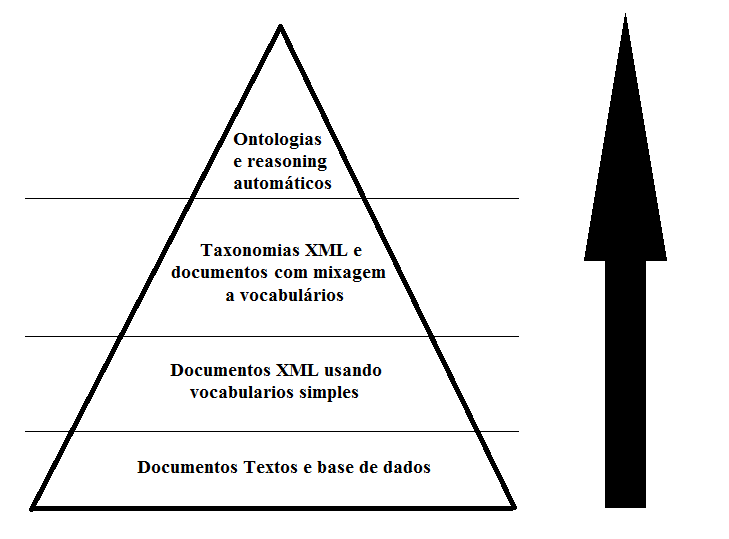
\includegraphics[width=12cm]{SmartDataContinuum.png}
    \caption{Níveis de Representação de Dados na forma de conhecimento processável por máquinas}
    \label{fig:RepresentacaoOntologia}
\end{figure}

O nível mais baixo de representação começa com os dados sem nenhum significado semântico, dependentes do contexto da aplicação. O segundo nível envolve a definição de esquemas XML para conseguir independência dos dados da aplicação, os dados fluem entre aplicações em um único domínio mas não podem ser compartilhados fora do domínio. No terceiro nível, os dados podem ser combinados a partir de diferentes domínios, sendo suficientemente independentes para serem recuperados e combinados com outras fontes de dados. Finalmente no quarto nível, é possível inferir novos dados a partir dos existentes e compartilha-los entre aplicações sem requerer interferência humana \cite{SugumaranGulla2011}, isso é possível graças as ontologias que descrevem esses dados. 

Uma ontologia é um sistema de organização e representação do conhecimento, em inglês \sigla{KOS}{Knowledge Organization System}, que é uma estrutura conceitual e computacional que permite representar o conhecimento, de qualquer domínio, por meio de entidades, classificações, relações semânticas, regras e axiomas.

Contudo, não existe um consenso sobre uma exata definição para ontologias. Segundo \cite{Gruber1995}, uma ontologia é "uma especificação explícita de uma conceitualização que representa o entendimento comum e a terminologia relevante de um domínio".

Uma ontologia é especificada por meio de componentes básicos que são as classes, relações, axiomas e instâncias. As classes, o foco da maioria das ontologias, são utilizadas para descrever os conceitos de um domínio, possibilitando a organização das classes em um sistema lógico e hierárquico contendo subclasses que representam conceitos mais específicos \cite{Noy2001}. As relações representam o tipo de interação entre os conceitos de um domínio e as propriedades presentes nas classes e indivíduos. Elas podem ter características próprias, como serem transitivas, simétricas, ou terem uma cardinalidade definida. Os axiomas são utilizados para modelar regras assumidas como verdadeiras no domínio em questão, de modo que seja possível associar o relacionamento entre os indivíduos, além de fornecer características descritivas e lógicas para os conceitos. Para \cite{UscholdGruninger1996} os axiomas são especificados para definir a semântica e significado dos termos (classes e propriedades) e sugerem que a fase de definição dos axiomas (especificação da ontologia) é a mais difícil na construção de ontologias. Por fim, os indivíduos, ou instâncias das classes, são utilizados para representar elementos específicos, ou seja, os próprios dados, que, juntamente com a definição de uma ontologia, constituem a base de conhecimento \cite{Noy2001}.


\section{Web Ontology Language}

A Web Ontology Language (OWL) foi recomendada pelo W3C em 2004 para representar e compartilhar ontologias na Web. Essa linguagem foi projetada para aplicações que necessitam processar o conteúdo da informação em vez de apenas apresentar informações em nós \cite{McGuinness2004}. OWL é uma linguagem que permite que semântica seja explicitamente associada ao conteúdo dos dados na web e formalmente especificada através de ontologias, compartilhadas na Internet.

A OWL 2, de abril de 2008, é a versão mais recente da linguagem 2. De acordo com as especificações do W3C\footnote{http://www.w3.org/TR/owl2-overview}, a OWL 2 adicionou três novos perfis (sub-linguagens) aos perfis DL e Full já existentes: OWL 2 EL, OWL 2 QL e OWL RL (\autoref{fig:OWLProfile}). Cada um desses perfis oferece um poder de expressividade diferente para diversos cenários de aplicação:

\begin{itemize}
    \item \textbf{FULL}: É direcionado para usuários que querem a máxima expressividade e a liberdade sintática do RDF sem nenhuma garantia computacional. É improvável que qualquer software de raciocínio seja capaz de suportar completamente cada recurso da OWL Full \cite{McGuinness2004}.

    \item \textbf{DL}: (Description Logic) é para aplicações que necessitam de máxima expressividade, enquanto mantém a computabilidade (todas as conclusões são garantidos para ser computáveis) e decidibilidade (todas as computações terminarão em tempo finito) \cite{McGuinness2004}. O OWL DL inclui todas as construções da linguagem OWL, mas elas podem ser usadas somente sob certas restrições.

    \item \textbf{EL}: É baseado na família EL++ de lógica descritiva (Description Logic), esse perfil é particularmente útil em aplicações utilizando ontologias que contêm um grande número de propriedades e/ou classes. Além disso, o OWL 2 EL utiliza um padrão comum utilizado em ontologias para conceitos e planejamento, ou seja, a combinação de conjunção e qualidades existenciais.

    \item \textbf{QL}: É baseado na família DL-Lite de lógica descritiva. Esse perfil foi criado para permitir o raciocínio (reasoning) eficiente com grandes quantidades de dados estruturados de acordo com esquemas relativamente simples. Ele fornece a maioria dos recursos necessários para capturar modelos conceituais, tais como diagramas de classe UML, diagramas de Entidade de Relacionamento, e esquemas de banco de dados.
 
    \item \textbf{RL}: É voltado para aplicações que exigem raciocínio escalável em troca de alguma restrição de poder expressivo. Ele define um subconjunto sintático de OWL 2 que favorece a implementação utilizando tecnologias baseadas em regras. Esse perfil pode ser utilizado na maioria das construções OWL 2, porém, para permitir implementações baseadas em regras de raciocínio, a forma como essas construções podem ser usadas em axiomas foi restringida.

\end{itemize}

\begin{figure}
    \centering
    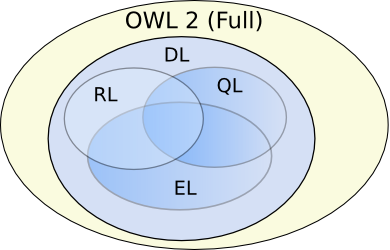
\includegraphics[width=12cm]{Owl2-profiles.png}
    \caption{OWL 2 Profiles}
    \label{fig:OWLProfile}
\end{figure}

Em um Sistema de Apoio a Decisão (SAD), ontologias podem ser usadas para modelar o domínio da aplicação deste sistema.
